\section{800 VDC MGX Architecture}

The above requirements for exponentially increasing power, pushing power out of the NVLink domain, and energy storage for mitigating load swings all come together to define the requirements for the 800 VDC power architecture.

\begin{figure}[h]
\centering
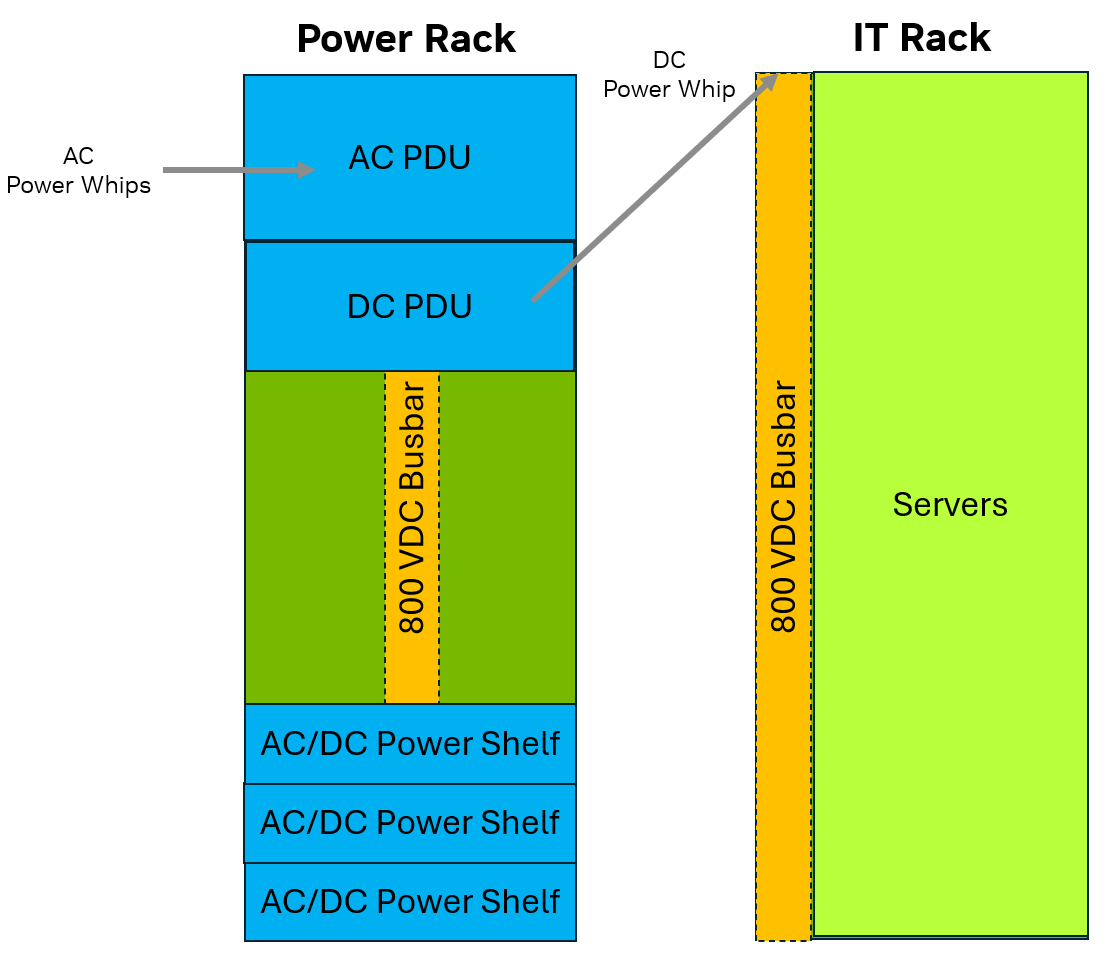
\includegraphics[width=0.8\textwidth]{figures/figure_p12_i1.png}
\caption{800 V MGX Rack Overview}
\label{fig:mgx-rack}
\end{figure}

The overall rack architecture takes 800 VDC directly into the rack and distributes 800 VDC direct to the compute node.

Safety is a critical design feature for the 800V system. Because of this touch-safe connectors are used in all locations that are user accessible. To ensure safety while connecting and disconnecting loads mechanical interlocks are also used in all connectors to ensure that there is no disconnect occurring under load. This helps to minimize the risk of arcing as well as act as a secondary protection ensuring that there are no live accessible parts. These techniques are commonly used in EV chargers which are widely available and used by untrained consumers. The presently planned connectors are leveraging this existing technology and optimizing for a datacenter environment.

To minimize connector sizes and volume of copper, the DC/DC conversion is pushed as close as possible to the GPU. This takes advantage of the 800 VDC to minimize power overhead in the system. The conversion is then done from 800 VDC to 12 VDC and routed a short distance to the voltage regulators.

The 800 VDC is converted directly to 12V with a 64:1 LLC converter and a matrix transformer. This helps to eliminate the separate 400V \textrightarrow{} 50V and 50V \textrightarrow{} 12V converters that are used in the present standard datacenter DC/DC converter power tree giving an additional 1\% in efficiency improvement and a 26\% reduction in area when compared to a multistage approach. This is in the critical area near the GPU.

\begin{figure}[h]
\centering
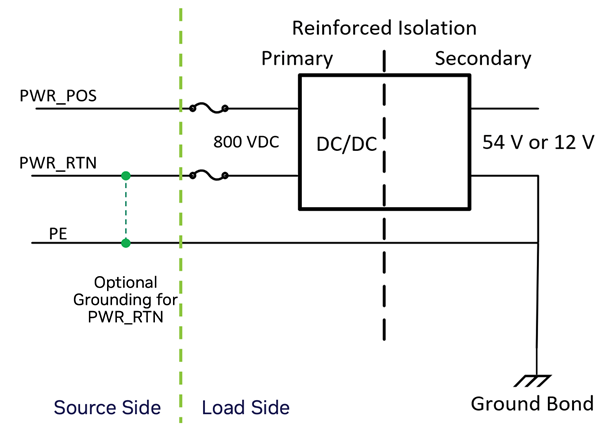
\includegraphics[width=0.8\textwidth]{figures/figure_p13_i1.png}
\caption{DC/DC with symmetrical fusing and hotswap controllers to allow for $\pm$400 VDC or 800 VDC sources}
\label{fig:dc-dc-fusing}
\end{figure}

The IT rack as shown in Figure~\ref{fig:dc-dc-fusing} is also designed to support sources with an 800 VDC total potential with multiple grounding schemes. This makes it so $\pm$400V equipment can be reused to power the rack. This is supported by having fuses on both the high side and low side input of the DC/DC converter and ensuring that both inputs have reinforced isolation from the secondary. To generate the 800 VDC powering the IT rack, there are multiple methods that can be used: side power racks, facility level rectification, medium-voltage rectifier and solid-state transformers.

The decision to implement an 800V DC single-ended configuration was driven by practical considerations around protection device availability and system simplicity when moving to datacenter level distribution. While bipolar configurations such as $\pm$400V DC offer theoretical benefits in grounding and fault isolation, they require specialized three-pole breakers and protection devices that are not widely available in the industry. Developing such components would introduce delays and increase engineering overhead. In contrast, the single-ended 800V DC approach aligns with existing two-pole breaker designs, allowing for faster deployment and reduced complexity. In addition, single ended distribution on the datacenter level does not have any load balancing issues across the positive and return sources.

\begin{figure}[h]
\centering
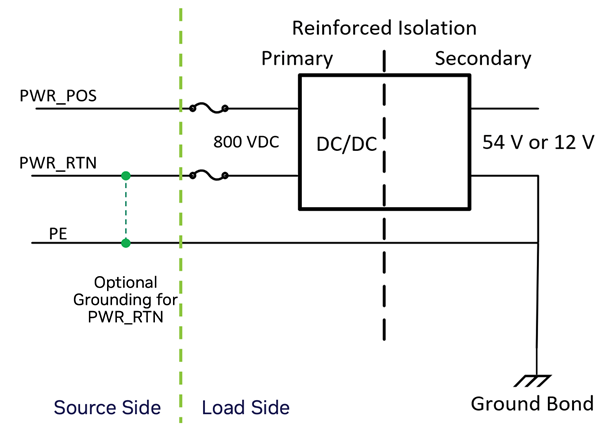
\includegraphics[width=0.8\textwidth]{figures/figure_p13_i1.png}
\caption{Datacenter architecture over time}
\label{fig:evolution}
\end{figure}

Figure~\ref{fig:evolution} illustrates the evolution of data center power distribution from the current 415 VAC architecture to future-ready 800 VDC systems designed to meet AI Factory demands. The existing 415 VAC architecture, shown in the top architecture, involves multiple components: MV step-down transformers, LV switchboards, AC UPS, PDUs, and AC distribution panels (RPP or busway). Power is delivered to each compute rack at 415 VAC, where an in-rack Power Shelf Unit (PSU) converts it to 54 VDC for compute trays and IT equipment. Optional external energy storage may be added to buffer dynamic power swings from the GPU workloads.

To support rising power densities and to provide an adapter to existing facilities, a transitional 800 VDC architecture relocates AC/DC conversion outside the rack. Targeting for White Space retrofit alone with minimal impact, an 800 VDC side power rack is a dedicated power rack containing rectifiers and power distribution units to convert from AC to DC local to each rack. This is required in the near term as components become more readily available to deploy 800 VDC datacenters. This is not the optimal solution end-to-end due to the extra stages of conversion, but it allows moving to higher compute rack densities by pushing power conversion out of the compute rack.

As 800 VDC power distribution equipment and data center operations become more readily available, the side power rack can be replaced by higher power density rectifier and being placed at the upstream of power distribution.

Facility-level AC/DC power rectifiers, as another variation, deliver 800 VDC from low-voltage AC (< 600 V). A typical rectifier string targets \textasciitilde{}1.5 MVA capacity and can be paralleled via a common DC bus. Positioned downstream of LV switchboards or directly under MV/LV transformers, these systems reduce rack-level complexity and support integration of energy storage at the DC output. While step-down transformers remain necessary, rectifiers offer mature, high-efficiency (\textasciitilde{}99\%) solutions widely used in BESS and renewables. This architecture simplifies power delivery and scales to support high-density compute with minimal white space burden.

To meet the rising power demands of AI Factories, NVIDIA is exploring MV Rectifier application (converting MV AC power to 800 VDC) and pursuing Solid State Transformer (SST) technology as future proof facility power distribution solutions. Shown in the bottom architecture, MV Rectifiers and SSTs are targeted to enable direct conversion from Medium Voltage (e.g., 35 kV AC) to 800 VDC, eliminating the need for traditional low-voltage (480 VAC) layers and simplifying the facility power architecture. Size of MV Rectifier and SST can be as large as 7.5 MVA per unit with 98.5\% or better efficiency.

A medium-voltage rectifier is a proven, high-capacity power conversion system widely used in industries like mining, electrolysis, rail, and grid-scale storage for delivering stable, high-power DC. Comprising a step-down transformer, rectification modules, filters, and protection systems, its mature design offers high reliability and supply chain readiness. Compared to the evolving SST, MV rectifiers provide a faster and proven path for quick 800 VDC deployment, making them a strong candidate for near-term AI Factory applications.

The SST system combines a medium-voltage AC intake, power rectification modules, and a DC output distribution section. Its compact and high-power capacity design supports compute rack density growth being scalable and great space saving with DC power equipment. However, scaling SSTs to multi-megawatt capacity presents challenges in the development and reliability of high-power rectification modules and managing thermal and electrical stresses at high density. NVIDIA is actively collaborating with leading industry partners to co-develop SST-based solutions.

The design of the facility-level DC power system must prioritize both resilience and scalability to meet the evolving needs of AI Factories. Resilience requires robust protection schemes, fault isolation strategies, and redundancy across power paths to ensure continuous operation during faults or maintenance. Scalability demands a modular and flexible architecture that enables seamless power expansion without major rework, while upholding safety and efficiency. Key development areas include high-capacity, reliable power rectification, advanced DC distribution boards, coordinated protection with DC devices, clearly defined isolation points for safe maintenance, simplified power interfaces to IT racks, and integrated DC energy storage to mitigate dynamic power swings. Together, these elements form the foundation for long-term reliability and operational agility in high-density compute environments.
